% !TeX root = ./document.tex
\documentclass[document]{subfiles}
\begin{document}

\chapter{Спектр и резольвента оператора}

\begin{definition}
    $X$ --- банахово, $T \in \B(X), Ix = x, x \in X$ --- тождественный оператор
    \[ \lambda \in \bC \quad V(\lambda) : \bC \rightarrow \B(X) \quad V(\lambda) = \lambda I - T \]
    Теперь множество комплексных чисел разбивается на 2 подмножества. $\lambda$ --- \textbf{регулярное значение}, если $V(\lambda)$ --- биекция [[ теорема Банаха ]] $\Rightarrow
    \: \exists (V(\lambda))^{-1} \in \B(X)$. 

    $\rho(T) = \{ \lambda \text{ --- регулярная } \}$ --- \textbf{резольвентное множество}
    \[ R(\lambda) : \rho(T) \rightarrow \B(X) \quad R(\lambda, T) = R(\lambda) = (V(\lambda))^{-1} \]
    $R$ --- \textbf{резольвента}
\end{definition}

Операторно-значная функция: комплексному числу сопоставляем оператор.

Откуда берется такое пугающее слово резольвента? Рассмотрим уравнение $\lambda x - Tx = y$. Если $\forall y \in X  \: \exists! x$ --- решение этого уравнения, 
то $\lambda$ --- регулярное значение, а уравнение --- разрешимо (resolve). Англо-саксонское слово проникло и сюда

\[ \sigma(T) = \bC \setminus \rho(T)  \text{ --- спектр оператора }\]

Посмотрим, из каких частей состоит этот спектр. Почему $V$ может быть не биекцией? В конечномерных пространствах он мог быть только не инъекцией, но в бесконечномерных 
может быть и не сюръекцией.

\begin{enumerate}
    \item $\sigma_p$ --- точечный спектр (p = point)
    \begin{gather*}
        \lambda \in \sigma_p(T) \text{ если } \Ker(\lambda I - T) \ne \seq{0} \\
        X_\lambda = \Ker(\lambda I - T), x \in X_\lambda \Leftrightarrow Tx = \lambda x
    \end{gather*}
        $\lambda$ --- собственное значение, $X_\lambda$ --- собственное подпространство 
    \item $\sigma_c(T)$ --- непрерывный спектр (c = continuous) 
    \begin{gather*}
        \sigma_c(T) = \seq{\lambda \in \bC, \Ker(\lambda I - T) = \seq{0}, (V(\lambda))(X) \text{ --- всюду плотен в } X} \\
         \text{ то есть } \overline{(\lambda I - T)(X)} = X
    \end{gather*}
    хоть и не биекция, но почти --- на всюду плотном множестве существует решение уравнения
    \item $\sigma_r(T)$ --- остаточный спектр (r = remainder)
           \[ \sigma_r = \seq{\lambda \in \bC: \Ker(\lambda I - T) = \seq{0}, \overline{\lambda I - T(X)} \subsetneq X } \] 
           образ $(V(\lambda))(X)$ не плотен в $X$
\end{enumerate}

\[ \sigma(T) = \sigma_p(T) \cup \sigma_c(T) \cup \sigma_r(T) \] 
части спектра не пересекаются

\begin{example}
    Если $\dim X < +\infty$, то $\sigma(T) = \sigma_p(T)$
\end{example}

\begin{theorem}[свойства резольвенты]
    $X$ --- банахово, $T \in \B(X), \: \lambda, \mu \in \rho(T)$
    \begin{enumerate}
        \item $R(\lambda) R(\mu) = R(\mu) R(\lambda)$
        \item $R(\lambda)-R(\mu)=(\mu-\lambda)R(\lambda)R(\mu)$ (тождество Гильберта) 
        \item $\lambda \in \bC, \abs{\lambda} > \norm{T} \Rightarrow \lambda \in \rho(T)$
        \item $\rho(T)$ --- открытое множество, $\mu \in \rho(T), \seq{\lambda \in \bC: \abs{\lambda - \mu} < \frac{1}{\norm{R(\mu)}}} \subset \rho(T)$
        \item $R(\lambda)$ --- непрерывная функция, то есть $\liml_{\lambda \to \mu} \norm{R(\lambda) - R(\mu)} = 0, \liml_{\lambda \to \infty} R(\lambda) = 0$
        \item $F \in (\B(X))^*, g(\lambda) = F(R(\lambda)), \lambda \in \rho(T) \Rightarrow g(\lambda)$ --- аналитическая в $\rho(T)$ (то есть $\exists g^\prime(\lambda))$
    \end{enumerate}
\end{theorem}

\begin{proof}[1]
    \begin{gather*}
        V(\lambda)V(\mu) = (\lambda I - T)(\mu I - T) = \\ 
        [[I \text{ коммутирует со всеми}]] = (\mu I - T)(\lambda I - T) = V(\mu)V(\lambda) \\
        AB = BA, \: A,B \in \B(X), \: \exists A^{-1}, B^{-1} \Rightarrow \\
        (AB)^{-1} = (BA)^{-1} \Leftrightarrow B^{-1}A^{-1} = A^{-1}B^{-1}
    \end{gather*}
\end{proof}

\begin{proof}[2]
    \begin{gather*}
        A^{-1} - B^{-1} = A^{-1}(B-A)B^{-1} \\
        A = V(\lambda) = \lambda I - T \quad B = V(\mu) = \mu I - T \\
        B - A = (\mu - \lambda) I \\
        \Rightarrow R(\lambda) - R(\mu) = R(\lambda)(\mu - \lambda)I \cdot R(\mu) = (\mu - \lambda)R(\lambda)R(\mu)
    \end{gather*}
    это рассужедние связано с утвержедниями об открытости множества обратимых операторов, об обратимости оператора, близкого к тождественному,
     и всё это мы будем сейчас использовать
\end{proof}

\begin{proof}[3]
    \begin{gather*}
        \lambda \in \bC, \abs{\lambda} > \norm{T} \\
        V(\lambda) = \lambda I - T = \lambda \left(I - \frac{1}{\lambda} T \right), 
        \norm{\frac{1}{\lambda} T} < 1 \\
         [[\text{ теорема об обратимости оператора, близкого к тождественному }]] \Rightarrow \\
        \exists \left( I - \frac{1}{\lambda}T \right)^{-1} \Rightarrow R(\lambda) = \frac{1}{\lambda} \left(I - \frac{1}{\lambda}T \right)^{-1}
    \end{gather*}
\end{proof}

\begin{proof}[4]
    \begin{gather*}
        A \in \In(X), \text{ то есть } A \text { обратим}, [[\text{ теорема об открытости } \In(X)]] \Rightarrow \\ 
        \norm{B-A} < \frac{1}{\norm{A^{-1}}} \Rightarrow B \in \In(X) \\
        A = \mu I - T \quad B = \lambda I - T \\
        \norm{A - B} = \abs{\lambda - \mu} \quad \abs{\lambda - \mu} < \frac{1}{\norm{R(\mu)}} \Rightarrow \: \exists B^{-1}, \text{ т.е. } R(\lambda), \text{ т.е. } \\
        \lambda \in \rho(T)
    \end{gather*}
\end{proof}

\begin{proof}[5]
    \begin{gather*}
        \norm{V(\lambda) - V(\mu)} = \abs{\lambda - \mu} \\
        \liml_{\lambda \to \mu} \norm{V(\lambda) - V(\mu)} = 0 \\
        \varphi : \In(X) \rightarrow \In(X) \quad \varphi(A) \coloneqq A^{-1} 
        \intertext{$\varphi$ --- непрерывное отображение, доказали в теореме об открытости $\In(X)$} 
        \Rightarrow \liml_{\lambda \to \mu} \varphi(V(\lambda)) = \varphi(V(\mu)) \Leftrightarrow \liml_{\lambda \to \mu} R(\lambda) = R(\mu)
        \intertext{теперь воспользуемся формулой, которую мы вывели в доказательстве пункта 3}
        \liml_{\lambda \to \infty} \frac{1}{\lambda} T = 0 \Rightarrow \liml_{\lambda \to \infty} \left(I - \frac{1}{\lambda} T \right) = I [[\text{по непрерывности } \varphi]] \Rightarrow \\
        \liml_{\lambda \to \infty} \left(I - \frac{1}{\lambda} T \right)^{-1} = I \Rightarrow \liml_{\lambda \to \infty} R(\lambda) = \liml_{\lambda \to \infty} \frac{1}{\lambda} \left(I- \frac{1}{\lambda}T\right)^{-1} = 0 \\
        R(\lambda) = \frac{1}{\lambda} \left(I - \frac{1}{\lambda} T \right)^{-1}
    \end{gather*}
\end{proof}

\begin{proof}[6]
    напишем просто тождество Гильберта
    \begin{gather*}
        \frac{R(\lambda)-R(\mu)}{\lambda - \mu} \stackrel{2}{=} \frac{(\mu-\lambda)R(\lambda)R(\mu)}{\lambda - \mu} = -R(\lambda) R(\mu) \underset{\lambda \to \mu}{\longrightarrow} - R(\mu)^2 \\
        \intertext{ура, у нас получилась аналитическая функция со значениями в банаховом пространстве. Но такого у нас еще не было, и чтобы не вводить новый объект, мы просто применим наш функционал}
        F \in (\B(X))^* \quad g(\lambda) = F(R(\lambda)) \\
        \frac{g(\lambda) - g(\mu)}{\lambda - \mu} = \frac{F(R(\lambda)) - F(R(\mu))}{\lambda - \mu} = F \left( \frac{R(\lambda) - R(\mu)}{\lambda - \mu} \right) \underset{\lambda \to \mu}{\longrightarrow} \\
        -F((R(\mu))^2) \Rightarrow \: \exists g^\prime(\mu) \: \forall \mu \in \rho(T)
    \end{gather*}
\end{proof}

Важная теорема, которая будет простым следствием из доказанных свойств

\begin{theorem}[компактность и не пустота спектра]
    $X$ --- банахово, $T \in \B(X) \Rightarrow \sigma(T)$ --- не пуст и компактен
\end{theorem}

Достаточно необычно, что для того чтобы показать непустоту спектра, нам понадобится ТФКП, математика всё-таки едина, ёлы-палы! 
\begin{theorem}[Лиувилль]
    Пусть $f(\lambda)$ --- аналитическая в $\bC$ и ограниченная, то есть $\exists M  > 0 : \abs{f(\lambda)} \leq M \: \forall \lambda \in \bC \Rightarrow f(\lambda) \equiv const$.
\end{theorem}

По секрету, функции, аналитические во всей комплексной плоскости, называются \textbf{целыми}.
\begin{proof}[Доказательство теоремы Лиувилля]
    \begin{gather*}
        a \in \bC \quad f^\prime(a) = \frac{1}{2\pi} \int_{\seq{|z-a| = r}} \frac{f(z)}{(z-a)^2} dz \Rightarrow
        \intertext{то есть продифференцировали формулу Коши. Когда функция у нас целая, мы $r$ можем взять любое}
        \Rightarrow \abs{f^\prime(a)} \leq \frac{1}{2\pi} \frac{M \cdot 2\pi r}{r^2} = \frac{M}{r} \underset{r \to \infty}{\longrightarrow} 0 \\
        \Rightarrow f^\prime(a) = 0 \: \forall a \in \bC \\
        \Rightarrow f(\lambda) = c \: \forall \lambda \in \bC, c \in \bC
    \end{gather*}
\end{proof}

\begin{figure}
    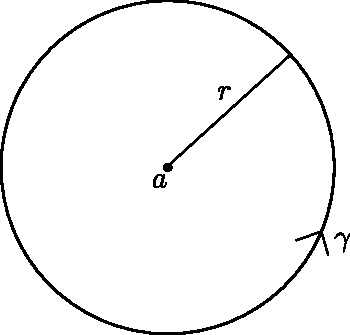
\includegraphics{chapter11/liuvill.pdf}\caption{Теорема 11.3}
\end{figure}

\begin{proof}[Доказательство теоремы]
    $\rho(T)$ --- открыто, $\rho(T) \subset \bC \Rightarrow \sigma(T) = \bC \setminus \rho(T)$ --- замкнутое. 
    \[ \abs{\lambda} > \norm{T} \Rightarrow \lambda \in \rho(T) \Rightarrow \sigma(T) = \seq{\lambda \in \bC: \abs{\lambda} \leq \norm{T}} \text{ --- ограниченное} \]
    $\Rightarrow \sigma(T)$ --- компакт.
    \begin{gather*}
        \text{пусть } \sigma(T) \ne \varnothing \Rightarrow \rho(T) = \bC \Rightarrow 0 \in \rho(T) \\
        V(0) = 0 \cdot I - T = -T, 0 \in \rho(T) \Rightarrow \: \exists T^{-1}
        \intertext{по следствию о достаточном числе линейных функционалов}
        \exists F \in (\B(X))^* : F(T^{-1}) = \norm{T^{-1}}, F(T^{-1}) \ne 0
        \intertext{но нас интересует только что $F(T^{-1}) \ne 0$}
        g(\lambda) = F(R(\lambda)) \quad \underline{g(0) \ne 0}, 6 \text{ свойство } \Rightarrow g(\lambda) \text{ аналитическая в } \bC  \\ 
        \liml_{\lambda \to \infty} R(\lambda) = 0 \Rightarrow \liml_{\lambda \to \infty} g(\lambda) = \liml_{\lambda \to \infty} F(R(\lambda)) = 0 \\
        [[\exists R > 0: \abs{g(\lambda)} \leq 1 \text{ при } \lambda \geq R, \exists M = \max_{|\lambda| \leq R} \abs{g(\lambda)} \Rightarrow \abs{g(\lambda)} \leq \max \{1, M \}]]
        \intertext{применяем теорему Лиувилля}
        g(\lambda) = const, \liml_{\lambda \to \infty} g(\lambda) = 0  \Rightarrow g(\lambda) \equiv 0 \Rightarrow \underline{g(0) = 0}\\
        \text{противоречие } \Rightarrow \sigma(T) \ne \varnothing
    \end{gather*}
\end{proof}

\begin{definition}[Спектральный радиус оператора $T$]
    $r(T) = \max_{\lambda \in \sigma(T)} \abs{\lambda}$. Из теоремы $\Rightarrow r(T) \leq \norm{T}$
\end{definition}
Примем без доказательства формулу
\[ r(T) = \liml_{n \to \infty} \sqrt[n]{\norm{T^n}} \] 

Наконец, обсудим, как связаны между собой спектр оператора и спектр сопряженного оператора.

\begin{theorem}[спектр сопряженного оператора]
    \begin{enumerate}
        \item $X$ --- банахово, $T \in \B(X) \Rightarrow$
            \begin{gather*}
                \sigma(T^*) = \sigma(T) \\
                \lambda \in \rho(T) \Rightarrow (R(\lambda, T))^* = R(\lambda, T^*)
            \end{gather*}
        \item $H$ --- гильбертово, $T \in \B(H), T^*$ --- эрмитово сопряженный 
            \begin{gather*}
                \sigma(T^*) = \seq{\overline{\lambda} : \lambda \in \sigma(T)} \\
                \lambda \in \rho(T) \quad R(\overline{\lambda}, T^*) = (R(\lambda, T))^*
            \end{gather*}
    \end{enumerate}
\end{theorem}

\begin{proof}[1]
    \begin{gather*}
        \left. \begin{matrix}
            \text{пусть } \lambda \in \rho(T) \Rightarrow \: \exists (\lambda I - T)^{-1} \\
            (\lambda I - T)^* = \lambda I - T^*
        \end{matrix} \right\} \Rightarrow \: \exists (\lambda I - T^*)^{-1} = ((\lambda I - T)^{-1})^*
    \end{gather*}
    В обратную сторону по замечанию \ref{chap10:remark} (из существования $(T^*)^{-1}$ следует существование $T^{-1}$)
\end{proof}

\begin{proof}[2]
    \[ (\lambda I - T)^* = \overline{\lambda} I - T^* \text{ и так далее} \]
\end{proof}

Маленькое ДЗ, которое когда-то давали в качестве задачи на 5 на экзамене
\begin{statement}
    $H$  --- гильбертово, $M$ --- замкнутое подпространство. $P : H \rightarrow M$ --- ортопроектор. $\sigma(P), R(\lambda)$ = ?
\end{statement}

Иногда кровожадные помощники задавали такие вопросы (но это не на 5, это просто на 1 секунду подумать): $I$ --- тождественный, $\sigma(I)$ = ?

\section{Компактные операторы}

\begin{definition}[компактный оператор]
    $X,Y$ --- банаховы, $T \in \Lin(X,Y)$. $T$ --- компактный, если $T(B^X_1(0))$ --- относительно компактен
\end{definition}

$\Com(X,Y)$ --- множество всех компактных операторов. Если $X=Y$, будем писать $\Com(X)$

\begin{remark}
    $\Com(X,Y) \subset \B(X,Y)$, $T(B^X_1(0))$ --- относительно компактно $ \Rightarrow T(B^X_1(0))$ --- ограниченное $\Rightarrow T \in \B(X, Y)$
\end{remark}

\begin{remark}
    $\forall A \subset X, A$ --- ограниченное, $T \in \Com(X,Y) \Rightarrow T(A)$ --- относительно компактно
\end{remark}

Понятно, что если есть относительная компактность образа единичного шара, то его можно раздувать как угодно.


Теперь еще один способ сказать, что оператор --- компактный. 
\begin{remark}
    $T \in \Com(X,Y) \Leftrightarrow \: \forall \seq{x_n}^\infty_{n=1} \text{ --- ограниченная } \Rightarrow \: \exists \seq{n_k}^\infty_{k=1} \text{ т. ч. } \exists \liml_{k \to \infty} T(x_{n_k}) = y_0 \in Y$
\end{remark}
Вот чем мы будем пользоваться изо всех сил: если последовательность ограниченная, то у нее есть сходящаяся в $Y$ подпоследовательность.

Более узкий класс операторов, но они же являются и примерами компактных операторов:
\begin{definition}[оператор конечного ранга]
    $X,Y$ --- банаховы, $T \in \B(X,Y), T$ --- \textbf{оператор конечного ранга}, если $\dim(T(X)) < +\infty$
\end{definition}

\begin{example}
    \begin{gather*}
        \seq{y_j}^n_{j=1}, y_j \in Y, \seq{f_j}^n_{j=1}, f_j \in X^* \\
        x \in X \quad Tx = \sum^n_{j=1} f_j(x) y_j \\
        \rank T = n
    \end{gather*}
\end{example}

Небольшое  ДЗ: показать, что любой оператор конечного ранга имеет такой вид.

\begin{statement}
    $T$ --- оператор конечного ранга $\Rightarrow T \in \Com(X, Y)$
\end{statement}

\begin{proof}
    $\dim(T(X)) < +\infty, T \in \B(X,Y) \Rightarrow T(B^X_1(0))$ --- ограниченное множество в конечномерном пространстве
     $\Rightarrow T(B^X_1(0))$ --- относительно компактно
\end{proof}

Существенная теорема о том, как связаны между собой компактность, операторы конечного ранга, конечномерные подпространства.

\begin{theorem}
    $X,Y$ --- банаховы, $T \in \Com(X,Y)$. Если $L = \overline{L}, L$ --- подпространство $T(X) \Rightarrow \dim L < +\infty$
\end{theorem}

\begin{proof}
    Первая часть доказательства. Допустим, что $L = T(X)$. Иными словами, предполагаем, что образ замкнут $\Rightarrow T(X)$ --- банахово как замкнутое подпространство полного пространства $Y$. Тогда вот что у нас есть
    \begin{gather*}
        T: X \rightarrow T(X) [[\text{ теорема Банаха об открытом отображении }]] \Rightarrow \\
        \exists B_r^{T(X)}(0) \subset T(B^X_1(0)) \text{ --- относительно компактно} \\
        \Rightarrow B_r^{T(X)}(0) \text{ --- относительно компактно} \\
        [[\text{ теорема Рисса }]] \dim(T(X)) < +\infty
    \end{gather*}
    Вторая часть, $L = \overline{L} \subset T(X)$, и тут другая идея, как это свести к предыдущему пункту. Рассмотрим $X_1 = T^{-1}(L), X_1$ --- банахово, потому что $T^{-1}$ --- непрерывный
    \[ T(X_1) = L, T \in \Com(X_1, L) \stackrel{1}{\Rightarrow} \dim L < +\infty \]
\end{proof}

\begin{corollary}
    $X$ --- банахово, $T \in \Com(X)$
    \begin{enumerate}
        \item Если $T(X) = X$, то $\dim X < +\infty$ 
        \item Если $\dim X = +\infty$, то $0 \in \sigma(T)$
    \end{enumerate}
\end{corollary}

\begin{proof}
    Первое очевидно. Второе от противного, предположим, что $0 \in \rho(T)$
    \begin{gather*}
        0 \in \rho(T) \Leftrightarrow V(0) = 0 \cdot I - T = -T, \: \exists T^{-1} \Rightarrow T(X) = X \text{ --- противоречие с 1} \\
        \Rightarrow 0 \in \sigma(T)
    \end{gather*}
\end{proof}

Посмотрим теперь, какие арифметические операции можно выполнять с компактными операторами

\begin{theorem}[арифметические операции и предельный переход в $\Com(X,Y)$]
    $X,Y$ --- банаховы 
    \begin{enumerate}
        \item $\Com(X,Y)$ --- замкнутое подпространство в $\B(X,Y)$. Поэтому будет сложение, композиция, умножение на константу и переход к пределу 
        \item $X \stackrel{T}{\rightarrow} Y \stackrel{S}{\rightarrow} Z, \: X, Y, Z$ --- банаховы
            \begin{enumerate}
                \item $T \in \B(X,Y), S \in \Com(Y,Z) \Rightarrow ST \in \Com(X,Z)$
                \item $T \in \Com(X,Y), S \in \B(Y,Z) \Rightarrow ST \in \Com(X,Z)$
            \end{enumerate}
    \end{enumerate}
\end{theorem}

\begin{proof}[1]
    \begin{gather*}
        T \in \Com(X,Y), \alpha \in \bC [[\text{ очевидно }]] \Rightarrow \alpha T \in \Com(X, Y) \\
        T, S \in \Com(X,Y) \quad B = B^X_1(0)
        \intertext{вспомним, что в полном пространстве относительная компактность эквивалентна вполне ограниченности}
        T(B) \text{ --- относительно компактно } \Leftrightarrow \text{ вполне ограничено}
        \intertext{хотим воспользоваться тем, что $T(B), S(B)$ --- вполне ограничены, а значит, $(S+T)(B)$ будет вполне ограниченным}
        \varepsilon > 0 \: \exists E \text{ --- конечная } \varepsilon\text{-сеть для } T(B) \\  
        \exists F \text{ --- конечная } \varepsilon\text{-сеть для } S(B) \\
        E + F = \seq{e + f : e \in E, f \in F} \text{ --- конечная } 2\varepsilon\text{-сеть для множества } T(B) + S(B) \\
        (T+S)(B) \subset T(B) + S(B) \\ 
        \Rightarrow (T+S)(B) \text{ --- вполне ограничено } \Rightarrow \text{ относительно компактно}
    \end{gather*}
    Проверим замкнутость $\Com(X,Y)$. Возьмём 
    \begin{gather*}
        \seq{T_n}^\infty_{n=1}, T_n \in \Com(X,Y) \\
        \liml_{n \to \infty} \norm{T_n - T} = 0
        \intertext{наша мечта проверить, что $T$ --- компактный оператор. Опять-таки воспользуемся вполне ограниченностью}
        \text{пусть } \varepsilon > 0 \: \exists n \in \bN : \norm{T_n - T} < \varepsilon \\
        \exists E \text{ --- конеченая } \varepsilon\text{-сеть для } T_n(B) \\
        \Rightarrow E \text{ --- } 2\varepsilon\text{-сеть для } T(B) \Rightarrow T(B) \text{ --- вполне ограничено}
    \end{gather*}
\end{proof}

\begin{proof}[2]
    $X \stackrel{T}{\rightarrow} Y \stackrel{S}{\rightarrow} Z, B = B^X_1(0)$

    Первый пункт: $T \in \B(X,Y) \Rightarrow T(B)$ --- ограниченное множество $\Rightarrow S(T(B))$ --- относительно компактно.

    Второй пункт: $T \in \Com(X,Y) \Rightarrow T(B)$ --- относительно компактен. $S$ --- непрерывное отображение $\Rightarrow S(T(B))$ --- относительно компактно.
\end{proof}

Вот какую умность можно сказать:
\begin{corollary}
    $X$ --- банахово, $\Com(X)$ --- замкнутый двусторонний идеал алгебры $\B(X)$
\end{corollary}

\section{Спектр компактного оператора}

Замечание-напоминание, которое, вероятно, было в алгебре, тут даже никакой непрерывности не требуется
\begin{remark}
    $X$ --- линейное пространство, $T \in \Lin(X), \seq{\lambda_j}^n_{j=1}, \lambda_j \ne \lambda_k$ при $j \ne k$
    \[ Tx_j = \lambda_j x_j, x_j \ne 0 \Rightarrow \seq{x_j}^n_{j=1} \text{ --- линейно независимы } \]
\end{remark}

\begin{theorem}
    $T \in \Com(X), X$ --- банахово, $\delta > 0$, $X_\lambda = \Ker(\lambda I - T)$ --- собственное подпространство, соответствующее $\lambda$
    \[ \sum_{\lambda \in \sigma_p(T), \abs{\lambda} > \delta} \dim X_\lambda< + \infty \]
\end{theorem}

Число линейно независимых собственных векторов, соотвествующих собственнным числам $\lambda$, таким, что $\abs{\lambda} > \delta$, конечно.

\begin{proof}
    Доказывать будем от противного. 
    \begin{gather*}
        \text{пусть } \seq{x_n}^\infty_{n=1} \text{ --- линейно назвисимы }, Tx_n = \lambda_n x_n, \abs{\lambda_n} > \delta
        \intertext{возможно, $\lambda_n = \lambda_m$ при $n \ne m$}
        L_n = \calL \seq{x_j}^n_{j=1}, L_n \subsetneq L_{n+1} \\
        [[\text{ следствие из леммы Рисса \hyperref[chap5:riss-corollary]{5.10}}]] \Rightarrow % ссылку 
        \exists \seq{y_n}^\infty_{n=1}, \norm{y_n} = 1, \rho(y_{n+1}, L_n) \geq \frac{1}{2} \\
        T \in \Com(X) \Rightarrow \: \exists \seq{n_k}^\infty_{k=1} \\
        \exists \liml_{k \to \infty} Ty_{n_k}
        \intertext{Проверим, что $\norm{Ty_n - Ty_m} > \varepsilon(\delta) > 0$, то есть не существует фундаментальной подпоследовательности}
        y_n = \alpha_n x_n + u_n, u_n \in L_{n-1} \\
        Ty_n = \alpha_n \lambda_n x_n + T u_n, Tx_j = \lambda_j x_j \Rightarrow T(L_n) \subset L_n
        \intertext{учёным образом говоря, $L_n$ --- инвариантное подпространство относительно оператора $T$}
        Ty_n = \lambda_n(\alpha_n x_n + u_n) - \lambda_n u_n + Tu_n = \lambda_n y_n + v_n, \: v_n \in L_{n-1} \\
    \end{gather*}
    сейчас докажем, что $\norm{Ty_n - Ty_m}$ отделена от нуля, это и есть наша мечта, это и будет противоречием.
    пусть $n > m$
    \begin{multline*}
        \norm{Ty_n - Ty_m} = \norm{\lambda_n y_n + v_n - Ty_m} = \abs{\lambda_n} \norm{y_n + \frac{1}{\lambda_n}(\underbrace{v_n}_{\in L_{n-1}} - \underbrace{Ty_m}_{\in L_{n-1} \text{т.к. } n > m})} \geq \\
        \delta \rho(y_n, L_{n-1}) \geq \frac{1}{2} \delta
    \end{multline*}
\end{proof}


Отметим такое тривиальное следствие
\begin{corollary}
    $X$ --- банахово пространство, $T \in \Com(X) \Rightarrow$
    \begin{enumerate}
        \item $\delta > 0, \# \seq{\lambda \in \sigma_p(T), |\lambda| \geq \delta} < +\infty$
        \item $\lambda \in \sigma_p(T), \lambda \ne 0 \Rightarrow \dim X_\lambda < +\infty$
        \item $\sigma_p(T) \setminus \{ 0 \} = \seq{\lambda_n}^N_{n=1}, 0 \leq N \leq +\infty$.
        Если $N = +\infty$, то $\liml_{n \to \infty} \lambda_n = 0$, можно занумеровать $|\lambda_1| \geq  |\lambda_2| \geq \ldots$
    \end{enumerate}
\end{corollary}
Всё очевидно, разве что про 3 что-то сказать. Вспоминаем одно из эквивалентных определений предела. Вот у нас есть 0, его $\delta$-окрестность, знаем что вне окрестности только конечное число элементов последовательности (это и утверждает теорема), а это и значит, что 0 --- предел.

\section{Самосопряжённые операторы}

\begin{theorem}[простейшие свойства самоспоряженного оператора]
    $H$ --- гильбертово, $T \in \B(H), T = T^*, ((Tx, y) = (x, Ty) \: \forall x, y \in H)$
    \begin{enumerate}
        \item $(Tx, x) \in \bR$ 
        \item $\lambda \in \sigma_p(T) \Rightarrow \lambda \in \bR$
        \item $\lambda, \mu \in \sigma_p(T), \lambda \ne \mu$, $Tu = \lambda u, Tv = \mu v \Rightarrow (u, v) = 0$
        \item $\norm{T} = \sup_{\seq{x: \norm{x} = 1}} \abs{(Tx, x)}$
        
    \end{enumerate}
\end{theorem}
Свойства 1--3 были доказаны в алгебре, вероятно, да и вообще доказываются в одну секунду. Будем считать их очевидными. Четвертый пункт самый содержательный

\begin{proof}[1]
       \[ (Tx, x) = (x, Tx)  = \overline{(Tx, x)} \Rightarrow (Tx, x) \in \bR  \]
\end{proof}
\begin{proof}[2]
    \[ \lambda \in \sigma_p(T) \Rightarrow \: \exists x > 0 : \: Tx = \lambda x \Rightarrow \] 
    \[ (Tx, x) = \lambda(x,x) \Rightarrow \lambda = \frac{(Tx,x)}{\norm{x}^2} \in \bR \]
\end{proof}

\begin{proof}[3]
    \begin{gather*}
        \lambda \ne \mu, \: \lambda, \mu \in \bR \text{ из (2)} \\
        (Tu, v) = (\lambda u, v) = \lambda(u, v) \\
        (Tu, v) = (u, Tv) = (u, \mu v) = \mu(u, v) \\
        0 = (\lambda - \mu)(u,v), \lambda \ne \mu \Rightarrow (u, v) = 0
    \end{gather*}
\end{proof}

\begin{proof}[4]
    \begin{gather*}
        Q = \sup_{\seq{x: \norm{x} = 1}} \abs{(Tx, x)}, \norm{x} = 1 \Rightarrow \\
        \abs{(Tx, x)} \leq \norm{Tx} \cdot \norm{x} \leq \norm{T} \cdot \norm{x}^2 = \norm{T} \\
        \forall x : \norm{x} = 1 \Rightarrow Q \leq \norm{T}
        \intertext{а в другую сторону нужно постараться}
        \text{пусть } u \in H, u \ne 0, \norm{\frac{u}{\norm{u}}} = 1 \Rightarrow \abs{\left( T\left(\frac{u}{\norm{u}}\right), \frac{u}{\norm{u}} \right)} \leq Q \Rightarrow \\
        \abs{(Tu, u)} \leq Q \norm{u}^2 \: \forall u \in H \\
        \text{пусть } x, y \in H, u = x + y \Rightarrow \\
        (T(x+y), x + y) \leq Q \norm{x+y}^2 \\
        -(T(x-y), x - y) \leq Q \norm{x+y}^2 \\
        \intertext{неравенства складывать можно, а вычитать нельзя, поэтому во втором неравенстве появился минус}
        (T(x+y), x + y) = (Tx, x) + (Ty, x) + (Tx, y) + (Ty, y) = \\
         [[ (Tx, y) = (x, Ty) = \overline{(Ty, x)}]] = \\
        = (Tx, x) + 2 \Real(Tx, y) + (Ty, y) \\
        (T(x-y), x-y) = (Tx, x) - 2 \Real(Tx, y) + (Ty, y)
        \intertext{вспомним тождество параллелограмма}
        \left.
        \begin{matrix}
            4 \Real(Tx, y) \leq 2Q(\norm{x}^2 + \norm{y}^2) \\
            \text{пусть } \norm{x} = 1, \text{ пусть } Tx \ne 0, y = \frac{Tx}{\norm{Tx}} \Rightarrow \norm{y} = 1
        \end{matrix} \right\} \Rightarrow \\
        4 \Real \left(Tx, \frac{Tx}{\norm{Tx}} \right) \leq 4Q \Rightarrow \norm{Tx} \leq Q \: \forall x, \norm{x} = 1 \\
        \Rightarrow \norm{T} = \sup_{\seq{x: \norm{x = 1}}} \norm{Tx} \leq Q
    \end{gather*}
\end{proof}

\begin{definition}[границы оператора]
    \[T = T^*,  M = \sup_{x: \norm{x} = 1} (Tx, x), m  = \inf_{x: \norm{x} = 1} (Tx, x) \] 
    $m, M$ --- границы оператора $T$
\end{definition}

\begin{remark}
    $T = T^* \Rightarrow \norm{T} = \max\{ |m|, M \}$
\end{remark}
Еще одна причина, почему <<границы>>
\begin{remark}[без доказательства]
    $T = T^* \Rightarrow \sigma(T) \subset [m, M]$
\end{remark}

Вот минимальные сведения о самосопряжённых операторах 

\section{Компактные самосопряжённые операторы}

\begin{theorem}
    $H$ --- гильбертово, $T \in \B(H), T \in \Com(H), T = T^*$
    \[ \Rightarrow \exists \lambda \in \sigma_p(T), \abs{\lambda} = \norm{T} \]
\end{theorem}

\begin{proof}
    \begin{gather*}
        M = \sup_{x: \norm{x} = 1} (Tx, x), m  = \inf_{x: \norm{x} = 1} (Tx, x) \\
        \norm{T} = \max\{ |m|, M \} \\
        \text{пусть } \norm{T} = M \quad \exists \seq{x_n}^\infty_{n=1}, \norm{x_n} = 1 \\
        M = \liml_{n \to \infty} (Tx_n, x_n), T \in \Com(H), \: \exists \seq{n_k}^\infty_{k=1} \text{ т.ч.} \\
        \exists \liml_{k \to \infty} Tx_{n_k} = y 
        \intertext{не умаляя общности, просто чтобы не писать много индексов, $\exists \liml_{n \to \infty} Tx_n = y$. Сейчас убедимся, что $y$ --- искомый собственный вектор, то есть $y \ne 0, Ty = My$}
        \norm{Tx_n} \leq \norm{T} \cdot \norm{x_n} = M \\ 
        \norm{y} = \liml_{n \to \infty} \norm{Tx_n} \Rightarrow \norm{y} \leq M \\
        0 \leq \norm{Tx_n - M x_n}^2 
    \end{gather*}
    наша мечта доказать, что эта разница стремится к нулю при $n \to \infty$
    \begin{multline*}
        \norm{Tx_n - M x_n}^2 = (Tx_n - Mx_n, Tx_n - Mx_n) = \underbrace{\norm{Tx_n}^2}_{\to \norm{y}^2} - \underbrace{M(Tx_n, x_n)}_{\to M^2} - \\
        - \underbrace{M(x_n, Tx_n)}_{\to M^2} + M^2\norm{x_n}^2 \underset{n \to \infty}{\longrightarrow} \norm{y}^2 - M^2 \\
        \Rightarrow \norm{y} \geq M \Rightarrow \norm{y} = M \Rightarrow y \ne 0
    \end{multline*}
        возвращаемся к тому, с чего начинали
        \begin{gather*}
        \Rightarrow \liml_{n \to \infty} Tx_n = M \cdot \liml_{n \to \infty} x_n \Rightarrow y = M \cdot \liml_{n \to \infty} x_n [[\text{ применим } T]] \Rightarrow \\
        Ty = M \cdot \underbrace{\liml_{n \to \infty} Tx_n}_{=y} \Rightarrow Ty = My \\
        \text{Если } \norm{T} = |m|, \: T_1 = -T \: \sup_{\seq{x: \norm{x} = 1}} (T_1x, x) = -m \\
        \text{уже показали, что } \exists y \ne 0: \: T_1 y = -my \Rightarrow Ty = my, \lambda \in \sigma_p(T), \lambda = m \\
        |\lambda| = \abs{m}
    \end{gather*}
    короче говоря, применим первую часть доказательства к $T_1$ и получим то, что надо
\end{proof}

\begin{theorem}[Гильберт-Шмидт]
    $H$ --- гильбертово, $T \in \Com(H), T = T^*, \sigma_p(T) \setminus \{0\} = \seq{\lambda_n}^N_{n=1}, 0 \leq N \leq + \infty$ 
    \begin{gather*}
        H_{\lambda_n} = \Ker(\lambda_n I - T), P_{\lambda_n} \text{ --- ортогональный проектор на } H_{\lambda_n} \\
        \Rightarrow T = \sum^N_{n=1} \lambda_n P_{\lambda_n}
    \end{gather*}
    если $N = +\infty$, то $\liml_{n \to \infty} \norm{T - \sum^n_{k=1} \lambda_k P_{\lambda_k}} = 0$
\end{theorem}

\begin{proof}
    Доказательство действительно напоминает то, как это делается в алгебре. Отщепляем собственные подпространства. Тут мы  ещё можем и перейти к пределу. 
    Сначала сделаем такое абстрактное действие 
    \begin{gather*}
        \lambda \in \sigma_p(T), \lambda \ne 0, \: H_\lambda = \Ker(\lambda I - T), \: P_\lambda : H \rightarrow H_\lambda \text{ --- ортпроектор }
        \intertext{и что за отщепление?}
        \widetilde{T} = T - \lambda P_\lambda
        \intertext{сейчас отметим,  что он самосопряженный, компактный, собственные числа и собственные подпространства такие же, как у оператора $T$. Обсудим подробнее связь 
        $T$ и $\widetilde{T}$}
        (\widetilde{T})^* = T^* - \overline{\lambda} P^*_\lambda = T - \lambda P_\lambda \text{ т.к. } \lambda \in \bR, T = T^*, P^*_\lambda = P_\lambda \\
        L \coloneqq H^\perp_\lambda \text{ то есть } H = H_\lambda \oplus L
        \intertext{так как $P_\lambda$ отправлят элементы из $L$ в 0, если  $x \in L = H_\lambda^\perp, \widetilde{T} = Tx-\underbrace{\lambda P_\lambda(x)}_0$, а 
        если $x \in H^\lambda, Tx = \lambda x, \widetilde{T}x = Tx - \underbrace{\lambda P_\lambda(x)}_{\lambda x}$}
        \widetilde{T} |_L = T, \widetilde{T} |_{H_\lambda} = 0  \\
        \text{пусть } \mu \in \sigma_p (T), \mu \ne 0, \mu \ne \lambda \Rightarrow H_\mu \perp H_\lambda \Rightarrow H_\mu \subset L \\
        \Rightarrow \mu \in \sigma_p(\widetilde{T}), \Ker(\mu I - \widetilde{T}) = H_\mu = \Ker(\mu I - T)
    \end{gather*}
    то есть отщепление никак не испортит остальные собственные числа и собственные подпространства
    \begin{gather*}
        \exists \lambda_1 \quad \lambda_1 \in \sigma_p(T), \abs{\lambda_1} = \norm{T}
        \text{так как мы знаем, что } \forall \lambda \in \sigma(T), |\lambda| \leq \norm{T} \\
        \lambda_1 \text{ имет наибольший возможный модуль} \\
        \intertext{если вдруг окажется, что $\lambda_1 = 0$, то $T = \bZero$. Тогда вообще непонятно, что утверждает теорема, ноль равен сумма пустого числа слагаемых... далее пусть $T \ne \bZero$}
        T_1 = T \quad T_2 = T_1 - \lambda_1 P_{\lambda_1} \\
        \text{если } T_2 = \bZero, \text{ то } T = \lambda_1 P_{\lambda_1} \\
        \text{если } T_2 \ne \bZero, \text{ то } \exists \lambda_2 = \norm{T_2} = \sup_{\seq{x: \norm{x} = 1}} \abs{(T_2x, x)} = \sup_{\seq{x: \norm{x} = 1, x \perp H_{\lambda_1}}} \abs{(Tx, x)} \\
        \text{и так далее } T_n = T - \lambda_1 P_{\lambda_1} - \ldots - \lambda_{n-1} P_{\lambda_{n-1}} \\
        \text{если } T_n = \bZero, \text{ то } T = \sum^{n-1}_{k=1} \lambda_k P_{\lambda_k} \\
        \text{если } \forall n \: T_n \ne \bZero \quad \norm{T_n} = \abs{\lambda_n} = \sup_{\seq{x: \norm{x} = 1, x \perp H_{\lambda_j}, 1 \leq j \leq n - 1}} \abs{(Tx, x)} \\
        \text{если } N = +\infty, \text{ то } \liml_{n \to \infty} \lambda_n = 0 \\
        \abs{\lambda_n} = \norm{T - \sum^{n-1}_{k=1} \lambda_k P_{\lambda_k}} \underset{n \to \infty}{\longrightarrow} 0 \\
    \end{gather*}
\end{proof}

\begin{theorem}[Гильберт-Шмидт]
    В сепарабельном гильбертовом пространстве у самосопряженного компактного оператора существует О.Н.Б из собственных векторов
\end{theorem}

Это та самая теорема, которая обещалась на первой лекции! Тут уже почти нечего доказывать.

Покороче: $H$ --- гильбертово, $T = T^*, T \in \Com(H) \Rightarrow \: \exists \seq{e_n}^\infty_{n=1} \text{ О.Н.Б. }, e_n$ ~--- собственные векторы.

\begin{proof}
    \begin{gather*}
        \sigma_p(T)  \setminus \{ 0 \} = \seq{\lambda_n}^N_{n=1}, 1 \leq N \leq +\infty \\
        H_{\lambda_n} = \Ker(\lambda_n I - T), m_n = \dim H_{\lambda_n} \\
        m_n < +\infty, \seq{e_{n, j}}^{m_n}_{j=1} \text{ --- О.Н.Б. в } H_{\lambda_n}
        \intertext{возьмём все векторы и рассмотрим замыкание линейной оболочки}
        L = \overline{\calL \seq{e_{n,j}}^N_{n=1, 1 \leq j \leq m_n}} \text{ --- замыкание линейной оболочки} 
        \intertext{используя предыдущую теорему, проверим, что $L = \overline{T(H)}$}
        Te_{n,j} = \lambda_n e_{n,j}, \lambda_n \ne 0 \Rightarrow e_{n,j} = T \left( \frac{e_{n,j}}{\lambda_n} \right) \Rightarrow L \subset \overline{T(H)}
        \intertext{а чтобы показать включение в другую сторону, понадобится предыдущая теорема}
        x \in H \text{ по предыдущей теореме} \: Tx = \sum^N_{n=1} \lambda_n P_{\lambda_n} x \Rightarrow Tx \subset L \Rightarrow T(H) \subset L \\
        P_{\lambda_n} x = \sum^{m_n}_{j=1} (x, e_{n,j}) e_{n,j}
        \intertext{$L$ --- замкнутое подпространство, поэтому нам ничего не стоит и замкнуть $(L = \overline{L}) \Rightarrow \overline{T(H)} \subset L$.
        $T(H)$ --- всегда есть О.Н.Б. из собственных векторов $H$ (для $\forall H$, не обязательно сепарабельного); уже доказазал для любого $T$}
        H = \overline{T(H)} \oplus \Ker T^* = \overline{T(H)} \oplus \Ker T, H_0 = \Ker(0 \cdot I - T) = \Ker T \Rightarrow \\
        H = L \oplus H_0 
        \intertext{$H$ --- сепарабельное $\Rightarrow H_0$ --- сепарабельное, $m_0 = \dim H_0, 0 \leq m_0 \leq +\infty$} 
        \seq{\lambda_{0,j}}_{j=1}^{m_0} \text{ --- О.Н.Б. в } H_0 \\
        \Rightarrow \seq{e_{n,j}}^N_{n=0, 1 \leq j \leq m_n} \text{ --- О.Н.Б. в } H
    \end{gather*}
\end{proof}

\begin{theorem}[о спектре компактного самосопряженного оператора]
    $H$ --- бесконечномерное гильбертово пространство, $T \in \Com(H), T = T^*$ 
    \[ \Rightarrow \sigma(T) = \sigma_p(T) \cup \{ 0 \} \] 
\end{theorem}

0 может быть собственным числом, а может и не быть. Остальные комплексные числа, не 0 и не собственные, являются регулярными. Начнём с тривиальной леммы. Раньше её вариант 
давался в качестве задачки на 5 на экзамене.

\begin{lemma}
    $\HCal$ --- сепарабельное гильбертово пространство, $\seq{e_n}^\infty_{n=1}$ --- О.Н.Б. 
        \[ \seq{\mu_n}^\infty_{n=1}, \mu_n \in \bC, Ae_n \coloneqq \mu_n e_n  \]
    продолжим по линейности на $\calL \seq{e_n}^\infty_{n=1}$
    \begin{enumerate}
        \item $A \in \B(\HCal) \Leftrightarrow \seq{\mu_n}^\infty_{n=1} \in l^\infty, \norm{A} = \norm{\seq{\mu_n}}_{l^\infty} = \sup_{n \in \bN} \abs{\mu_n}$ 
        \item $\exists A^{-1} \in \B(\HCal) \Leftrightarrow \inf_{n \in \bN} \abs{\mu_n} = \delta > 0$
    \end{enumerate}
\end{lemma}

\begin{proof}[Доказательство первого утверждения леммы]
    $\Rightarrow$ \\
    \begin{gather*}
        A \in \B(\HCal) \Rightarrow \norm{A} = \sup_{\seq{x: \norm{x} = 1}} \norm{Ax} \geq \norm{Ae_n} = \abs{\mu_n}  \: \forall n \\
        \Rightarrow \seq{\mu_n} \in l^\infty, \norm{A} \geq {\norm{\seq{\mu_n}}}_{l^\infty}
    \end{gather*}
        $\Leftarrow$
        \begin{gather*}
        x \in \HCal \Rightarrow x = \sum^\infty_{n=1} x_n e_n \Rightarrow \norm{x}^2 = \sum^\infty_{n=1} \abs{x_n}^2 \\
        \norm{Ax}^2 = \sum^\infty_{n=1} \abs{\mu_n}^2 \abs{x_n}^2 \leq \norm{\seq{\mu_n}}^2_\infty \norm{x}^2 \Rightarrow \norm{A} \leq \norm{\seq{\mu_n}}_\infty
    \end{gather*}
\end{proof}

\begin{proof}[Доказательство второго утверждения леммы]
    \[ A^{-1} e_n = \frac{1}{\mu_n} e_n \: \text{ из 1 } A^{-1} \in \B(\HCal) \Leftrightarrow \seq{\frac{1}{\mu_n}} \in l^\infty \Leftrightarrow \inf_{n \in \bN} \abs{\mu_n} > 0 \] 
\end{proof}

\begin{proof}[Доказательство теоремы]
    \begin{gather*}
        \seq{\lambda_n}^N_{k=1} = \sigma_p(T) \setminus \{ 0 \} \\
        E = \sigma_p(T) \cup \{ 0 \} \Rightarrow E \text{ --- замкнутое}
        \intertext{$E$ замкнуто, поскольку если последовательность конечная, то и обсуждать нечего, а если бесконечная, то их предельная точка обязательно 0}
        \lambda \notin E \: \exists \delta > 0 \: \abs{\lambda - \lambda_n} \geq \delta, \abs{\lambda} \geq \delta \\
        H_{\lambda_n}, \seq{e_{n,j}}^{m_n}_{j=1} \text{ --- О.Н.Б. в } H_{\lambda_n} \\
        x \in H \: x = x_0 + x_1, x_0 \in H_0 \quad x_1 \in L = \overline{T(H)} \\
        Tx = \underbrace{Tx_0}_{=0} + Tx_1 = \sum^N_{n=1} \lambda_n \sum_{j=1}^{m_n} (x, e_{n,j}) e_{n,j}
        \intertext{мечтаем доказать, что у $(\lambda I - T)$ есть обратный}
        (\lambda I - T)x = \lambda x_0 + \sum^N_{n=1} (\lambda - \lambda_n) \sum^{m_n}_{j=1} (x, e_{n,j}) e_{n,j} \\
        \abs{\lambda - \lambda_n} \geq \delta, \abs{\frac{1}{\lambda-\lambda_n}} \leq \frac{1}{\delta}, \seq{\frac{1}{\lambda-\lambda_n}} \in l^\infty [[\text{ лемма }]] \Rightarrow \\
        \exists R(\lambda) = (\lambda I - T)^{-1} \\ 
        (\lambda I - T)^{-1} y = \frac{1}{\lambda} y_0 + \sum^N_{n=1} \frac{1}{\lambda-\lambda_n} \sum^{m_n}_{j=1} (y, e_{n,j}) e_{n,j}
    \end{gather*}
\end{proof}

\begin{remark}[без доказательства]
    $X$ --- банахово бесконечномерное, $T \in \Com(X) \Rightarrow \sigma(T) = \sigma_p(T) \cup \seq{0}$
\end{remark}

\section{Интегральный оператор в $L^2$}

Это главный пример оператора, к которому применяют эти все теоремы Гильберта-Шмидта.

\begin{theorem}
    $X \subset \bR^n, Y \subset \bR^m, X, Y$ --- измеримые по мере Лебега множества. 
       \[  K(x,y) \in L^2(X \times Y, dx dy_{\text{ в } \bR^{m+n}}) \]
    \[ \left( \int_X \int_Y \abs{K(x,y)}^2 dxdy \right)^{\frac{1}{2}} < +\infty \] 
    \[ (\K f) (x) = \int_Y K(x,y) f(y) dy, f \in L^2(Y) \] 
    $\Rightarrow \K \in \Com(L^2(Y), L^2(X))$
\end{theorem}

\begin{proof}
    Докажем, что $\norm{\K} \leq \norm{K(x,y)}_{L^2(X \times Y)}$.
    Идея такая: будем приближить этот компактный оператор операторами конечного ранга. Мы знаем, что они компактные и мы знаем, что можно переходить к пределу. А предел компактных
    операторов --- компактный оператор.
    \begin{gather*}
        L^2(X) \text{ --- сепарабельное } \Rightarrow \exists \seq{\varphi_n(x)}^\infty_{n=1} \text{ О.Н.Б. в } L^2(X) \\
        L^2(Y) \text{ --- сепарабельное } \Rightarrow \exists \seq{\psi_m(x)}^\infty_{m=1} \text{ О.Н.Б. в } L^2(Y) \\
       \int_X \varphi_n(x) \overline{\varphi_m(x)} dx = \begin{cases}
            0 & n \ne m \\
            1 & n = m
        \end{cases}
        \intertext{проверим $\seq{\varphi_n(x) \psi_m(y)}_{n, m \in \bN}$ --- О.Н.Б. в $L^2(X \times Y)$} 
        \int_X \int_Y \varphi_n(x)  \psi_m(y) \overline{\varphi_k(x)} \overline{\psi_j(y)} dxdy = \begin{cases}
            1 & n = k, m = j \\
            0 & (n,m) \ne (k, j)
        \end{cases}
        \intertext{проверим полноту теперь через критерий: предположим, что есть функция, которая ортогональна этой системе}
        \seq{\varphi_n \psi_m} \text{ --- полная в } L^2(X \times Y): \text{ пусть } f(x,y) \in L^2(X \times Y), f \perp \seq{\varphi_n \psi_m} \: \forall n, m \\
        \int_X \int_Y f(x,y) \overline{\varphi_n(x)} \overline{\psi_m(y)} dxdy = 0 \: \forall n, m \\
        \text{ пусть } n \text{ --- фиксированное } \\
        \int_Y \left( \int_X f(x,y) \overline{\varphi_n(x)} dx \right) \overline{\psi_m}(y) dy = 0
        \intertext{есть некоторая фиксированная функция, ортогональная всем элементам базиса $\psi_m$} 
        \Rightarrow \int_X f(x,y) \overline{\varphi_n(x)} dx = 0 \text{ п.в. } y \in Y \\
        \text{ для п.в. } y \text{ для } \forall n \in \bN \quad \int_X f(x,y) \overline{\varphi_n}(x) dx = 0 \Rightarrow
        \intertext{аналогично заключаем, что и $f(x,y) = 0$ почти всюду}
        f(x,y) = 0 \text{ п.в. } x \in X \Rightarrow f = \bZero \text{ в } L^2(X \times Y) \Rightarrow \\
        \seq{\varphi_n(x) \psi(m)y} \text{ --- базис в } L^2(X \times Y)
        \intertext{теперь разложим ядро по базису}
        K(x,y) \in L^2(X \times Y) \Rightarrow \\
        K(x,y) = \sum_{1 \leq i, j < +\infty} \alpha_{ij} \varphi_i(x) \psi_j(y) \\
        K_n(x,y) = \sum_{1 \leq i, j \leq n} \alpha_{ij} \varphi_i(x) \psi_j(y), \norm{K(x,y) = K_n(x,y)}_{L^2} \underset{n \to \infty}{\longrightarrow} 0  
    \end{gather*}
    идея такая: рассмотрим интегральный оператор с ядром $K_n$, убедимся, что он конечного ранга, значит, он будет компактным, а потом перейдем к пределу, поскольку в множестве 
    компактных операторов можно переходить к пределу, оператор с ядром $K$ тоже будет компактным оператором
    \begin{multline*}
        f \in L^2(Y), (\K_n f)(x) = \int_Y K_n(x,y) f(y)dy = \int_Y \sum_{1 \leq i, j \leq n} \alpha_{ij} \varphi_i(x) \psi_j(y) f(y) dy = \\
        = \sum_{1 \leq i, j \leq n} \alpha_{ij} \varphi_i(x) \int_Y \psi_j(y) f(y) dy \in \calL(\varphi_i(x))^n_{i=1}
    \end{multline*}
    \begin{gather*}
        \dim \K_n(L^2(Y)) = n < +\infty \\
        \Rightarrow \K_n \text{ --- оператор конечного ранга } \\
        \Rightarrow \K_n \in \Com(L^2(Y), L^2(X))
    \end{gather*}
    мы учились оценивать норму интегрального оператора с помощью нормы его ядра
    \begin{gather*}
        \norm{\K - \K_n}_{\B(L^2(Y), L^2(X))^*} \leq \norm{K(x,y)- K_n(x,y)}_{L^2(X,Y)} \underset{n \to \infty}{\longrightarrow} 0 \\
        \Rightarrow \K \in \Com(L^2(Y), L^2(X))
    \end{gather*}
\end{proof}

Отметим такое следствие, главный пример, к которому применяются теоремы Гильберта-Шмидта
\begin{corollary}
    $X \subset \bR^n, X$ --- измеримое, $K(x,y) \in L^2(X \times X)$
    \[ K(y,x) = \overline{K(x,y)} \quad (\K f)(x) = \int_X K(x,y) f(y) dy \: f \in L^2(X) \] 
    \[ \Rightarrow \K = \K^*, \K \in \Com(L^2(X)) \] 
    к оператору $\K$ применили теорему Гильберта-Шмидта. Верно не только для меры Лебега
\end{corollary}

\section{Каноническое представление компактного оператора}
Произвольный компактный оператор нет надежды представлять такой замечательной суммой, поскольку у него может быть только одно собственное число --- 0, 
и весь спектр будет состоять из 0, и ничего не напишешь больше.
\begin{definition}
    $H$ --- гильбертово, $T \in \B(H), T = T^*, T \geq 0 \text{ если } (Tx, x) \geq 0 \: \forall x \in H$
\end{definition}
$S = S^*, S \geq T$ если $S - T \geq 0$

\begin{example}
    \[ T = T^*, m = \inf_{\seq{x: \norm{x} = 1}} (Tx, x), M = \sup_{\seq{x: \norm{x} = 1}}(Tx, x) \]
    $Ix = x, mI \leq T \leq MI$
\end{example}

\begin{theorem}
    $H$ --- гильбертово, $T \in \B(H) \Rightarrow$ 
    \begin{enumerate}
        \item $TT^* \geq 0$ 
        \item $\norm{TT^*} = \norm{T}^2$
        \item $\Ker(T^*T) = \Ker T$
    \end{enumerate}
\end{theorem}

Теорема хороша тем, что $T$ произвольный, и мы можем рассмотреть $TT^*$, и он уже будет положительно определённый и самосопряжённый

\begin{proof}[1]
    \begin{gather*}
        (TT^*)^* = TT^* \Rightarrow TT^* \text{ --- самосопряжённый} \\
        (TT^*x, x) = (T^*x, T^*x) = \norm{T^*x}^2 \geq 0
    \end{gather*}
\end{proof}

\begin{proof}[2]
       \[ \norm{x} = 1 \quad \norm{TT^*} = \sup_{\seq{x: \norm{x} = 1}} \abs{(TT^*x, x)} = \sup_{\seq{x: \norm{x} = 1}} \norm{T^*x}^2 = \norm{T}^2 \]
\end{proof}

\begin{proof}[3]
    \begin{gather*}
        Tx = 0 \Rightarrow T^*Tx = 0 \\
        \text{пусть } T^*Tx = 0 \Rightarrow (T^* Tx, x) = 0 \Rightarrow \underbrace{(Tx, Tx)}_{=\norm{Tx}^2} = 0 \Rightarrow Tx = 0
    \end{gather*}
\end{proof}

Из того, что оператор положительно определённый, следует, что его собственные числа неотрицательные.
\begin{remark}
    $\mu_n \geq 0$ 
    \[ (Tx, x) \geq 0 \: \forall x \in  H, Tx = \lambda x \Rightarrow \lambda = \frac{(Tx,x)}{\norm{x}^2} \geq 0 \] 
\end{remark}

\begin{definition}[сингулярное число оператора]
    $T \in \Com(H), H$ --- гильбертово $\Rightarrow T^* T \in \Com(H), (T^*T)^* = (TT^*) \Rightarrow \sigma_p(T^*T) \setminus \{0\} = \seq{\mu_n}^N_{n=1}$,
    $\mu_n \geq 0, \mu_1 > \mu_2 > \ldots$, если $N=+\infty$, то $\liml_{n \to \infty} \mu_n = 0$
    \[ s_n = \sqrt{\mu_n} \] 
    $s_n$ --- сингулярное число оператора $T$
\end{definition}

$m_n = \dim(\mu_n I - T^* T), m_n$ --- кратность сингулярного числа $s_n$

\begin{theorem}[каноническое разложение компактного оператора]
    $H$ ---гильбертово, $T \in \Com(H), \seq{s_n}^N_{n=1}$ --- сингулярные числа, $\seq{m_n}^N_{n=1}$ --- кратности $\Rightarrow$ 
    \[ \seq{e_{n,j}}^N_{n=1, 1 \leq j \leq m_n} \text{ --- О.Н.С., } \seq{f_{n,j}}^N_{n=1, 1 \leq j \leq m_n} \text{ --- О.Н.С., } \] 
    \[ Tx = \sum^N_{n=1} s_n \sum_{j=1}^{m_n} (x, e_{n,j}) f_{n,j} \] 
\end{theorem}
Наибольший интерес теорема представляет в случае бесконечных рядов $1 \leq N \leq +\infty$

\begin{proof}
    \begin{gather*}
        H_{\mu_n} = \Ker(\mu_n I - T^* T), m_n = \dim H_{\mu_n} \\
        \seq{e_{n,j}}^{m_n}_{j=1} \text{ --- О.Н.Б. в } H_{\lambda_n} \\
        f_{n,j} = \frac{1}{s_n}Te_{n,j} 
        \intertext{проверим, что они ортогональны друг другу}
        (f_{n,j}, f_{m,k}) = \frac{1}{s_n s_m} ( T e_{n,j}, Te_{m,k}) = \frac{1}{s_n s_m}(T^*T e_{n,j}, e_{m,k}) = \frac{\mu_n}{s_ns_m}(e_{n,j}, e_{m,k}) = \\ =
        \begin{cases}
            1 & n = m, j = k \\
            0 & (n, j) \ne (m, k)
        \end{cases} \\
        x = \underbrace{x_0}_{\in H_0} + \sum^N_{n=1} \sum_{j=1}^{m_n} (x, e_{n,j}) e_{n,j} \quad x_0 \in \Ker(T^*T) = \Ker(T) \\
        Tx = \sum^N_{n=1} s_n \sum^{m_n}_{j=1}(x, e_{n,j}) f_{n,j}
    \end{gather*}
\end{proof}

\begin{corollary}
    $T \in \Com(H), H$ --- гильбертово $\Rightarrow$ $\exists \seq{T_n}^\infty_{n=1}, T_n$ --- конечного ранга $\liml_{n \to \infty} \norm{T_n - T} = 0$
\end{corollary}

\begin{proof}
    Пусть $N= +\infty$, иначе оператор и так конечного ранга.
    \begin{gather*}
        T_nx = \sum^n_{k=1} s_k \sum^{m_k}_{j=1} (x, e_{k,j}) f_{k,j}, \text{ пусть } \norm{x} = 1 \\
        \norm{(T-T_n)x}^2 = \sum^\infty_{k=n+1} |s_k|^2 \left( \sum^{m_k}_{j=1} \abs{(x,e_{k,j})}^2 \right) \leq \abs{s_{n+1}}^2 \cdot \norm{x}^2 \leq \abs{s_{n+1}}^2 \underset{n \to \infty}{\longrightarrow} 0 
    \end{gather*}
\end{proof}

Конец.


\end{document}